\chapter{BeagleSNES Subsystems}

\section{Overview}\index{Overview}

\begin{updateWarn}
This section is currently BB-xM only.  It must be rewritten to include BBB information.  The overall concepts are still the same, though.
\end{updateWarn}

BeagleSNES uses the Simple DirectMedia Layer (SDL)\footnote{\texttt{http://www.libsdl.org}} library to provide audio, video, and input event functionality for both the game selection menu and the emulator.  SDL is a cross-platform library which has a simple programming interface that abstracts away many of the details involved when creating multimedia applications.  The BeagleSNES emulator is based on an SDL port of SNES9X\footnote{The original SNES9X-SDL source, prior to the BeagleSNES modifications, can be fetched from the Git repository at: \texttt{https://github.com/domaemon/snes9x-sdl}}.  The mainline version of SNES9X only supports an X11 video display target, which is unsuitable for the framebuffer video of BeagleSNES.  By using the SDL port, BeagleSNES is able to support a variety of interfaces, including those offered by the the BB-xM platform.

While the game selection menu and the emulator are really two separate applications (after all, the only purpose of the game selection menu is to provide the emulator with the filename of the ROM to be loaded), both exist in the same binary.  Early testing showed that there was a visible screen flicker and a delay of several seconds when transitioning from one to the other when each was broken out as a separate binary.  Therefore, the game selection menu will initialize all of the needed SDL subsystems (audio, video, and joystick), execute, and then shut down the audio and joystick subsystems prior to transitioning to the emulator.  The emulator will then reinitialize the audio and joystick subsystems while leaving the video subsystem alone\footnote{SDL allows an application to change the video resolution on-the-fly without reinitializing the video subsystem.  When the game selection menu and the emulator used to use different screen resolutions, the emulator had to change the resolution when it began executing.  But, it did not need to restart the video subsystem to do so.}.  By not shutting down the video subsystem and reinitializing it, the visible screen flicker is removed.
 
\section{Audio Subsystem}\index{Audio Subsystem}

The BeagleSNES audio subsystem uses the ALSA\footnote{The Advanced Linux Sound Architecture.  Read more about it at: \texttt{http://www.alsa-project.org}} interface that is exposed by kernel.  The interface is provided by the system-on-chip (SoC) audio driver for boards that have TWL4030 audio CODEC hardware\footnote{This audio driver is located in the file \texttt{sound/soc/omap/omap-twl4030.c} in the kernel source tree.}.  SDL offers an ALSA back-end, so many of the details involved in interfacing with ALSA are abstracted away from BeagleSNES by SDL. 

The game selection menu uses a helper library, SDL\_mixer\footnote{\texttt{http://www.libsdl.org/projects/SDL\_mixer}}, to provide an even simpler interface to SDL's audio subsystem.  SDL\_mixer allows BeagleSNES to easily fade music in and out, load audio in a variety of formats, and mix several channels of audio together.  SDL only provides a standard interface for pushing audio data out to the audio driver back-end, so the more advanced functionality of SDL\_mixer provides the additional features needed to create a full-featured audio solution.

BeagleSNES configures the audio hardware of the BB-xM to use signed 16-bit stereo audio samples with a sampling rate of 32000 Hz.  Both the game selection menu and the emulator use these same audio settings for simplicity.  The audio subsystem is initialized in the game selection menu so that audio feedback and background music\footnote{The background music that is played behind the menu comes from the group ViRiLiTY.  It was originally the tracked background music of an illicit serial number generator used for the piracy of the "ALO Power Audio Converter" software.} can be played while the end-user examines the list of games that are available for play.  

When a game is launched from the menu, any playing audio fades out and the audio subsystem is shut down.  The emulator then reinitializes the audio subsystem using its original program logic.  The emulator's implementation of the SNES's audio DSP performs all of the audio mixing, so SDL\_mixer is no longer needed.  While the real SNES hardware will play audio at almost the same time that its DSP generates the audio data, the BeagleSNES emulator has audio latency of approximately 100 ms.  This is caused by the time needed to place the generated DSP audio into the kernel's circular audio buffer and the time needed before the pre-existing audio data ahead of the new data in the buffer is consumed.  In practice, this delay is hardly ever noticed.  This latency can be reduced by shrinking the size of the kernel audio buffer (12000 bytes), but this increases the amount of CPU resources dedicated to refilling the buffer and risks the possibility of an audio buffer underrun.


\section{Video Subsystem}

BeagleSNES system's video output is displayed via the BB-xM's DVI digital output.  The initial release of BeagleSNES used the S-Video analog output for NTSC video output, but this ended up being a poor choice for the following reasons: 

\begin{itemize}
\item The analog video signal is very noisy.  The horizontal sync varies from scanline to scanline, there is a lot of static, and the color quality is poor.  Whether this is due to poor drivers or poor hardware quality is unknown.
 \item The 720x482 NTSC resolution is larger than what is needed for BeagleSNES.  This means that more pixels are being updated than are actually needed, which degrades performance.
\item During development, profiling of BeagleSNES showed that displaying the framebuffer was much slower for the analog output than it was for the digital output.
\item The NTSC analog output has a refresh rate of 29.97 Hz, while the DVI digital output has a refresh rate of 60 Hz.  This means that the digital output can potentially display at a rate of 60 FPS, while the analog signal artificially limits the frame rate to half that amount.
\item NTSC signals suffer from overscan.
\end{itemize}

\noindent{}All components of BeagleSNES render their graphics to the framebuffer console, which is set to a native resolution of 640x480 and a color depth of 16 BPP.  These particular settings are hard-coded into the "omapfb" framebuffer driver\footnote{This framebuffer video driver is located in the file \texttt{drivers/video/omap/omapfb\_main.c} in the kernel source tree.} within BeagleSNES's Linux kernel. The refresh rate of 60 Hz means that whatever data is present in the framebuffer is pushed out as a single frame of video and is displayed for roughly 0.0167 seconds.  At the end of that time period, the data in the framebuffer will then be pushed out as the next single frame of video.

The emulator runs at a logical 60 FPS internally, but this does not necessarily mean that it will render video at 60 FPS.  The emulator can potentially skip the rendering of many frames of video if it falls behind schedule and needs to make up the difference.  The skipped frames will not even be noticed in many cases, though performance-intensive titles that require a large amount of CPU time to emulate the SNES hardware will not have enough CPU time left to perform the rendering of enough frames each second to make the gameplay "smooth".

\subsection{Video During Boot}\index{Video Subsystem}

One of the defining characteristics of a consumer-oriented embedded device is that it "turns on" immediately after it is powered up.  The device must give the consumer some indication that it is now going through its start-up process.  Displaying some sort of graphical splash screen immediately after power up is an excellent way to achieve this.  Unfortunately, BeagleSNES does not provide such a splash screen.  Or, at least, it does not do so immediately upon powering up.  To do so would require adding functionality to the BeagleSNES bootloader to display the splash screen\footnote{There actually is preliminary support for a splash screen in the bootloader, but it has not been "hooked up" yet and needs further testing.}. 

Roughly five seconds after power up, a much simpler method to display a splash screen becomes available.  At that point in time, the bootloader has loaded, decompressed, and begun bootstrapping the kernel.  The kernel initializes the graphical framebuffer and displays the first graphical output of the system: an 80x80 pixel, 224 color image of Tux the Penguin.  This icon is displayed in the upper left corner of the framebuffer console.  BeagleSNES turns this image into a splash screen by replacing the original image\footnote{This image is located at \texttt{drivers/video/logo/logo\_linux\_clut224.ppm} in the kernel source tree.} with a much larger image: a 640x480 pixel, 224 color image of the BeagleSNES logo.

\begin{figure}[h]
\centering
\includegraphics[scale=0.28]{video_chapter/boot_splash.png} 
\includegraphics[scale=0.28]{video_chapter/beaglesnes_kernel_splash.png}
\caption{The original BeagleSNES's splash screen (left) was the smallest size it could be (640x300) for NTSC (720x482), but the current one (right) is the same size as the screen resolution (640x480) for simplicity.}
\end{figure}

Even though BeagleSNES uses a full-screen splash image, it is not really necessary for the splash screen to be the full resolution of the screen.  The background color of the framebuffer is black, and the image is displayed in the upper left corner of the screen, so it is only necessary to include the bare minimum amount of splash screen image needed to center the BeagleSNES logo on the screen.  The splash screen is compiled into the kernel, so a smaller image reduces both the size of the kernel and the time it takes for the bootloader to load the kernel into memory from the microSD card.  Adding a splash screen in this fashion increases the compressed kernel's size by only about 20kb.  Normally, debug and information messages are printed to the framebuffer console as the kernel boots, but BeagleSNES suppresses the printing of these messages\footnote{These messages can still be viewed via the serial debug interface (\texttt{/dev/ttyO2}), though.} so that they do not overwrite the splash screen image.

The splash screen remains on the screen while the kernel continues to bootstrap.  Once it is finished, the splash screen disappears as the "icon" in the upper left corner is removed.  The screen remains blank until the game selection menu appears approximately 17-18 seconds after power-up.
 
\subsection{Game Selection Menu}\index{Video Subsystem}

The BeagleSNES game selection menu uses the entire 640x480 screen. The video subsystem of SDL is used to request an SDL video surface to render to.  This surface is not requested using the SDL\_FULLSCREEN flag, even though the resolution we want to use is the entirety of the screen.  Profiling the use of SDL\_FULLSCREEN has shown that it is much slower than not using it, so it is always better for BeagleSNES to use a "windowed" mode for all of its framebuffer graphics.  For the simple animations of the menu, though, the impact of slower execution is minimal.

When BeagleSNES used analog video, not all of the space on the screen was usable. Due to NTSC overscan, some portion of the edges of the screen may be "cut off" by the television that the image is being displayed on. The amount that is cut off varies depending upon the particular television, so it is important to design the interface so that there is a "safety buffer" around the edges of the screen where text and other important items must not be placed.  Typically, no more than a few pixels are cut off on each edge, though the left edge of the screen loses far more: a cut off of 12-16 pixels is common.  Digital video does not have this issue.

\begin{figure}[h]
\centering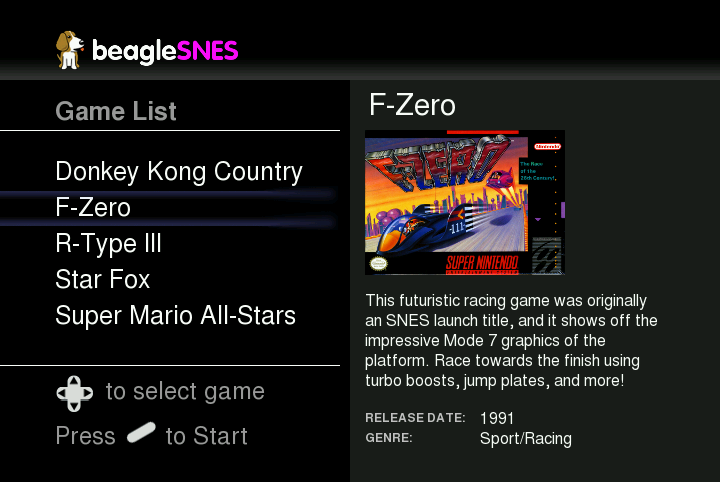
\includegraphics[scale=0.28]{video_chapter/gui_no_overscan.png} 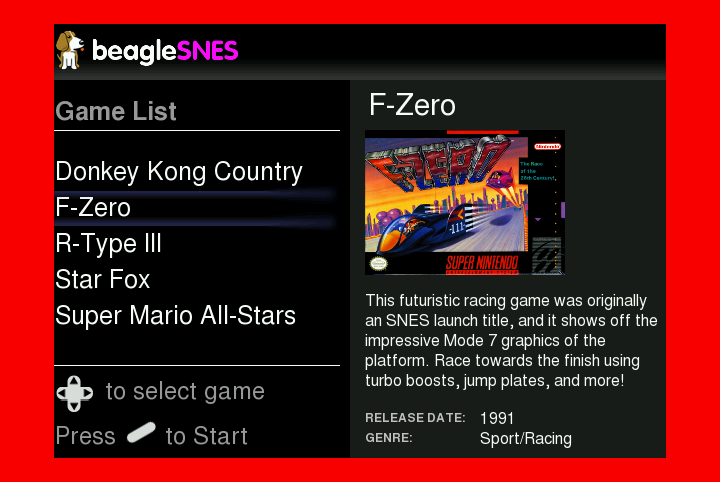
\includegraphics[scale=0.28]{video_chapter/gui_overscan.png}
\caption{A screenshot of the old game selection menu (left), and the same menu with the potential NTSC overscan regions marked in red (right).}
\end{figure}

\subsection{Emulator Execution}\index{Video Subsystem}

\emph{NOTE:} This section contains information about the video of the emulator from when BeagleSNES used analog video output.  It remains in the documentation because it may be of some technical interest to other BeagleBoard developers.

\emph{<Analog video material begins here>}

Once a selection has been made via the game selection menu, the screen fades to black prior to starting the emulator. This was not a choice based upon aesthetics (well, not directly, anyway). Internally, the emulator requests a 616x478x16 SDL video surface to render to. This resolution is different than what was previously set, so the SDL video subsystem actually has to be reconfigured with the new resolution. If the framebuffer is completely black, the transition between resolutions is never noticed by the end user. It also ensures that portions of the screen that are never updated by the emulator's rendering remain black during its execution.

The odd 616x478 resolution of the emulator was determined by the following method. Internally, each rendered scanline of SNES graphics is 512 pixels long. If we subtract the 512 pixels from the 720 pixel screen width, we have 208 pixels left in each scanline of the screen framebuffer (the screen framebuffer has a pitch of 1440 bytes, or (720 pixels * 2 bytes), so there are no extra offscreen pixels). If we divide these 208 pixels in half (since half will fall to the left of our SNES data and half will fall to the right of it), we have 104 pixels. 512 pixels + 104 pixels = 616 pixels, which is the resolution we request. Since we are not requesting a full-screen SDL video mode (via the SDL\_FULLSCREEN flag when calling SDL\_SetVideoMode()), the SDL surface will render into the left-most 616 pixels of the screen. With the offset of 104 pixels, the 512 pixels of the SNES scanline will render in the center of the screen. The emulator renders at a vertical resolution of 478 pixels. It is actually rendering each of the SNES's internal 239 scanlines twice to pixel double up to 478 scanlines. The SDL surface will render into the top-most 478 pixels of the screen, leaving the bottom 4 scanlines of the framebuffer untouched. Some, if not all, of these 4 scanlines will never even be seen, since they are usually lost to overscan.

\emph{<Analog video material ends here>}

Finally, by using an SDL\_UpdateRect() call to only update the portion of the framebuffer containing the 512x478 portion of SNES image data, we leave the chunks of black in the framebuffer that are to the left and right of the SNES graphics untouched. Why go to all of this trouble? Speed. There is a considerable difference between the speed of using the SDL\_FULLSCREEN mode (slow) and using only a portion of the screen (much faster). Titles that would run at close to 30 FPS would drop to 8-12 FPS when running in a full screen mode.

\section{Input Subsystem}\index{Input Subsystem}

BeagleSNES uses USB gamepad events as its only method for receiving input from the end user.  Both SDL and the Linux kernel view these gamepads as a USB human interface device (HID) class joystick devices.  SDL's input event mechanism for gamepads is split over two subsystems: video and joystick.  The video subsystem captures most events that are experienced by SDL-based applications: keyboard, mouse, window manager, etc..  Once the video subsystem is initialized, SDL's internal event queue is initialized as well.  Joystick events (the type of event that would be received from a gamepad) are an optional addition to the SDL event mechanism.  They are not received by the general SDL event handling code until the joystick subsystem is initialized.  Once that initialization occurs, gamepad events are also generated and placed into SDL's event queue alongside the other types of events.  

When the joystick subsystem is initialized, the underlying limitations of the Linux kernel's joystick interface become apparent.  The number of connected joysticks is reported, and any reported joysticks can then be "opened" to begin receiving events from them.  Unfortunately, there are \emph{many} things that could go wrong:

\begin{itemize}
\item If the USB hardware is unreliable (connections to devices are lost, but then quickly restored), SDL will stop responding to it.  This is because the "old" joystick is gone, but a "new" one has taken its place, and the new joystick must then be opened to use it.  
\item Joystick devices vary in the number of axis and buttons that the device provides to the software.  If an end-user plugs in a USB joystick device that reports a different number of buttons or axes, or reports buttons that are mapped in a different order than expected, then the behavior of the device will not be correct.
\item There are no "new joystick plugged in" or "joystick unplugged" events generated by SDL. There is only a mechanism to query how many joystick devices are currently plugged into the system.
\end{itemize}
 
BeagleSNES does its best to work around these limitations.  There is a known problem that the BB-xM has with briefly losing power to its USB devices.  This problem has the same effect as rapidly unplugging and then plugging in a gamepad: the gamepad appears to stop working because the joystick driver device file in the file system that SDL listens to for joystick events becomes invalid.   BeagleSNES addresses this problem with a kernel patch\footnote{This patch is for 3.2+ kernels.  Older kernels still suffer from this issue.} that properly handles this issue. 

Originally, BeagleSNES required that all gamepads must be plugged in prior to power up and not removed during system operation.  This situation is far from ideal, since gamepads can accidentally become unplugged during use.  The current approach to this problem is to tie the internal representation of a particular gamepad to the physical USB port on the system that the gamepad is plugged into.  Two of the BB-xM USB ports are designated explicitly for BeagleSNES gamepad use: one being the port for "player one" gamepad and the other for "player two".  Unless a gamepad is plugged into either of those particular ports (i.e. the "player one" or "player two" port), it will be completely ignored.  

When a USB gamepad is plugged into the BB-xM, new files are dynamically created in the \texttt{/sys} and \texttt{/dev} directories of the root file system, thanks to the \texttt{sysfs} support in the kernel\footnote{\texttt{sysfs} is a virtual file system that is accessible from user space.  It exports information about devices that are registered with the kernel, as well as a variety of driver information.  By reading these files from user space applications, the devices that these files represent can be interacted with easily.}.  Plugging a USB gamepad into the "player one" port creates a file\footnote{\texttt{/dev/input/by-path/platform-ehci-omap.0-usb-0:2.2:1.0-joystick}}, as does plugging a USB gamepad into the "player two" port\footnote{\texttt{/dev/input/by-path/platform-ehci-omap.0-usb-0:2.4:1.0-joystick}}.  Each of these files is a symbolic link to one of the \texttt{/dev/input/jsX} joystick device files.  These device files are opened from user space applications to access joystick events. By watching the creation and destruction of these files via a \texttt{stat()} or \texttt{readlink()} function call, BeagleSNES can determine whether a gamepad is present or not in those particular physical USB ports.  

The \texttt{/dev/input/jsX} device files enumerate the various joystick devices that are connected to the system, in the order that they are connected, using the device files \texttt{js0}, then \texttt{js1}, etc.  BeagleSNES will dynamically remap joystick events so that the events are attributed to the correct gamepad.  On each pass through the event handler loop, the "player one" and "player two" \texttt{sysfs} files are examined to see if they exist.  If either has changed, the joystick subsystem of SDL is shut down and restarted to reconfigure the gamepads accordingly.  This expensive operation only occurs if a controller has been plugged in or unplugged.  Otherwise, the only overhead created is by the two checks to see if the \texttt{sysfs} files exist and a table lookup to remap joystick events to the correct gamepad as those events occur.
